% !TEX root = ../thesis.tex
% appendix NXP KMZ60 char dataset
% @author Tobias Wulf
%

\chapter{NXP KMZ60 Kennfelddatensatz 0.0.1 29.03.2021}\label{ch:kmz60-datensatz}


\begin{figure}[tbph]
	\centering
	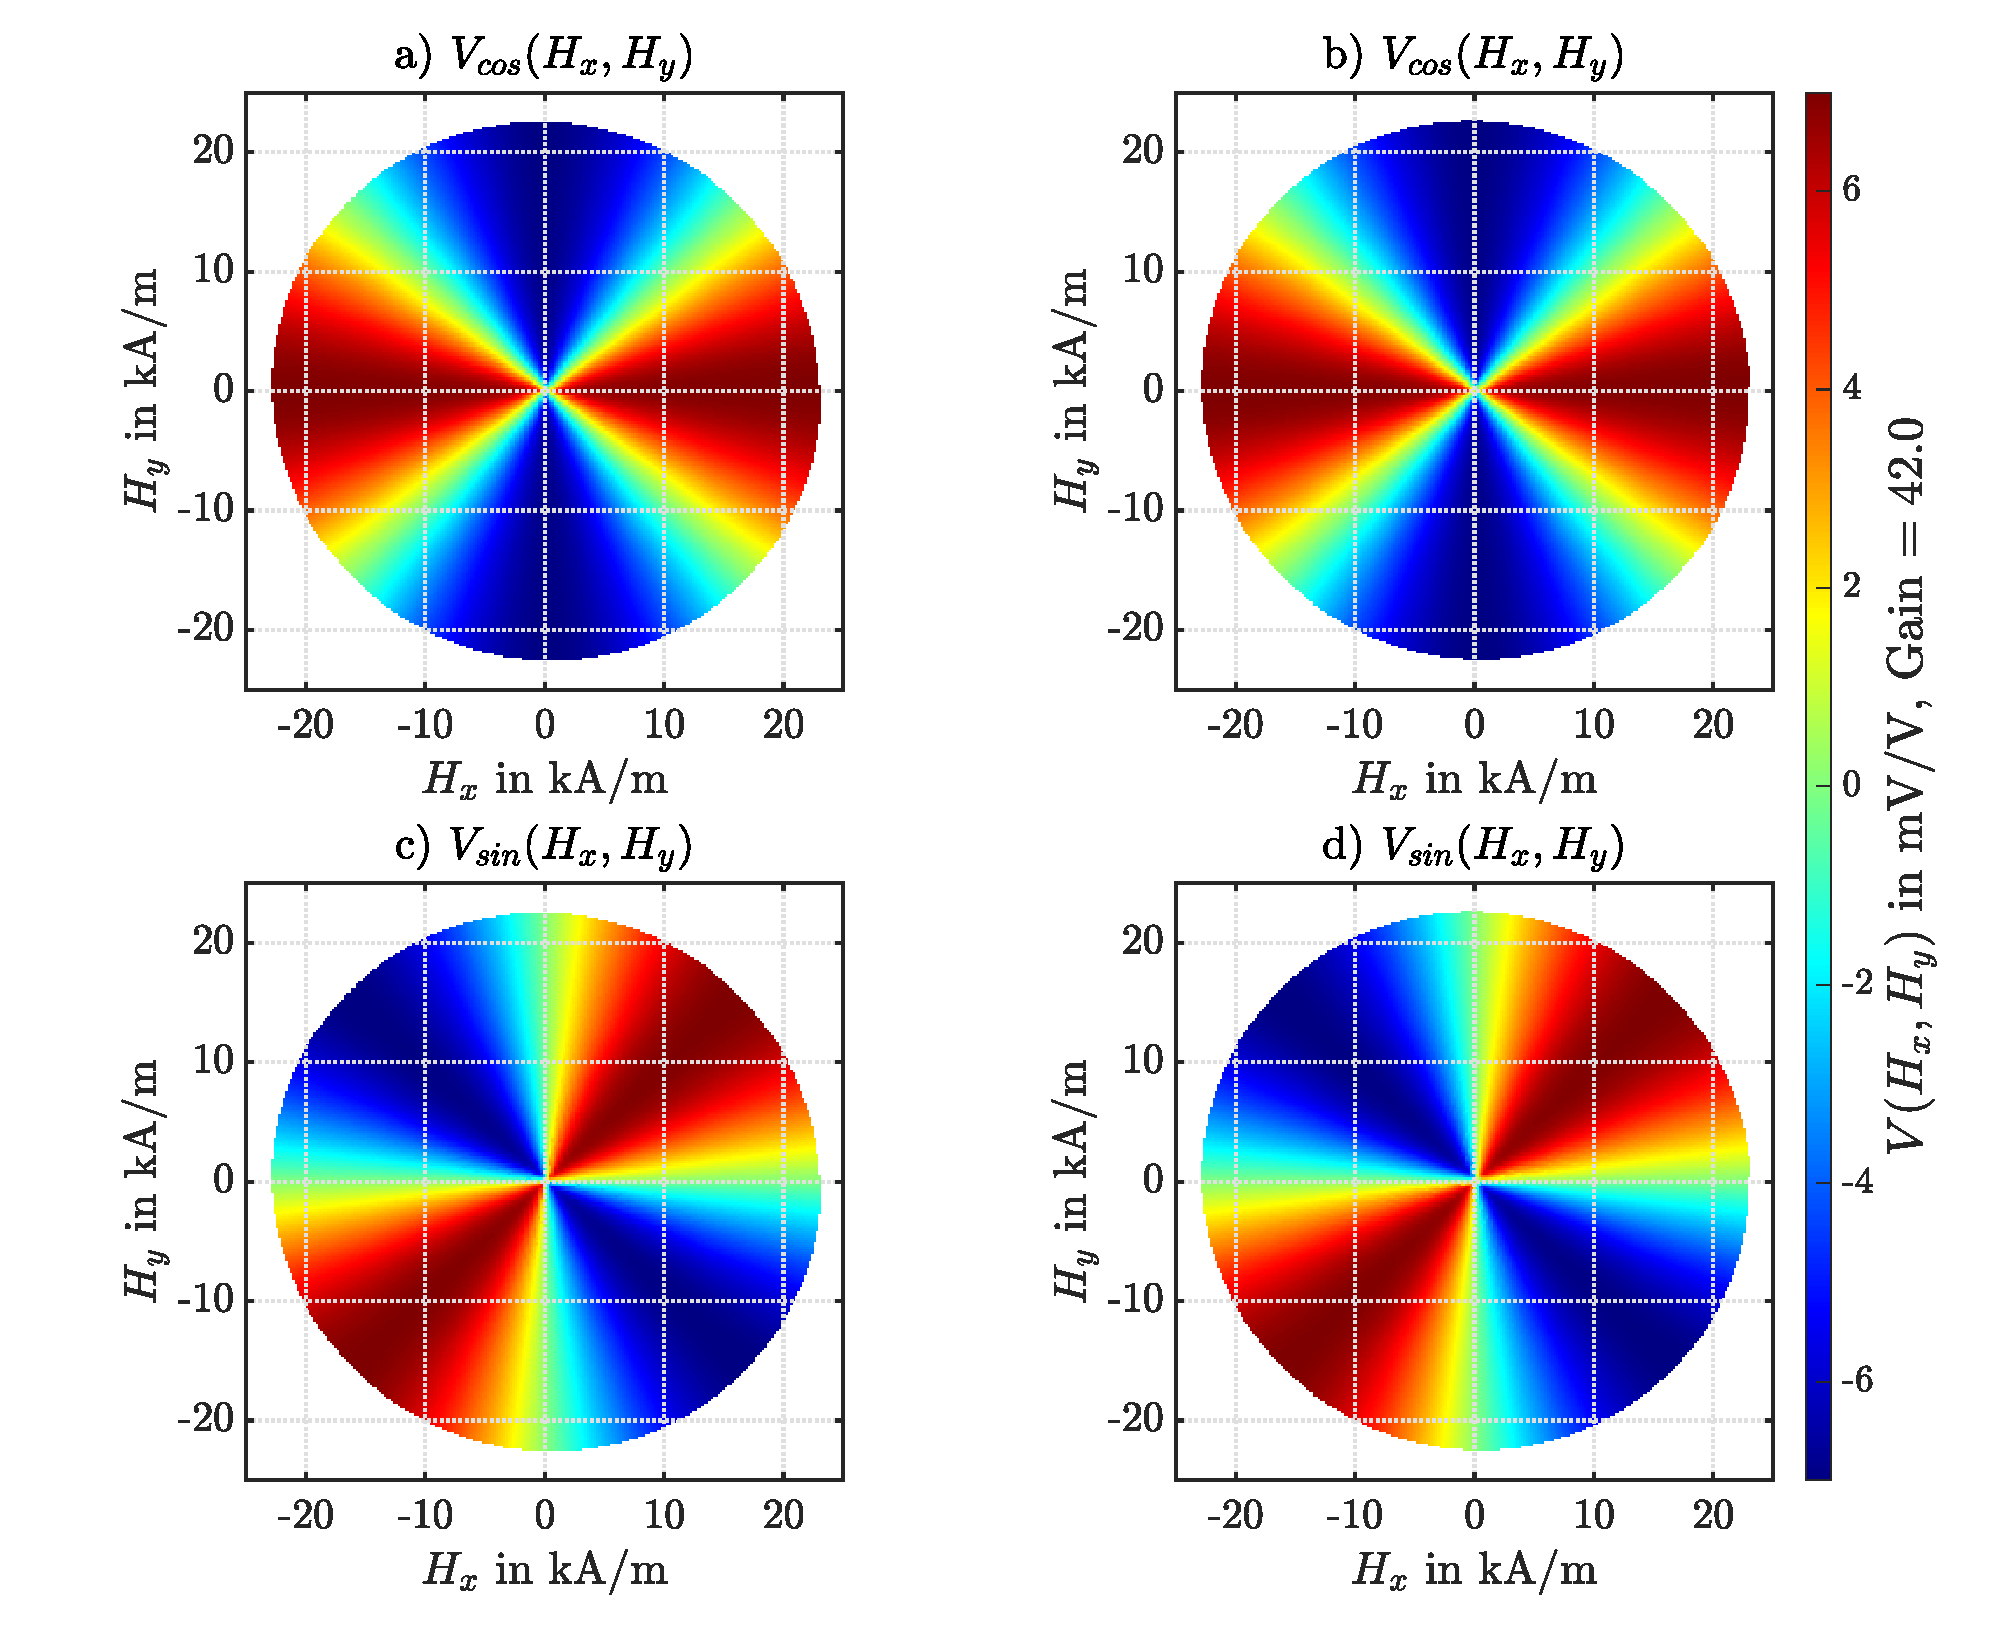
\includegraphics[width=\linewidth]{appendix/images/4-KMZ60/KMZ60_Kennfelder}
	\caption[NXP KMZ60 Winkelsensorbrückenkennfelder]{NXP KMZ60 Winkelsensorbrückenkennfelder. Zu sehen sind die 
		Kennfelder der Cosinus-Brücke a) und b). Darunter befinden sich die Kennfelder der Sinus-Brücke c) und d). 
		Die Kennfelder für beide Brücken a) und c) beziehen sich auf die steigenden Flanke der Amplitudenmodulation aus 
		\autoref{fig:magnetfeldstimuluskennfeldmethode} und die in b) bzw. d) gezeigten Kennfelder sind gewonnen aus 
		der fallenden Flanke. Die Brückenkennfelder sind normiert in $\SI{}{\milli\volt\per\volt}$. Für eine 
		Spannungsausgabe in Betriebsspannungsniveau ist eine zusätzliche Verstärkung um Faktor $42$ notwendig. Die 
		Kennfelder besitzen, jeweils in $H_x$- und $H_y$-Richtung, eine Schrittweite von 
		$\SI{0.1961}{\kilo\ampere\per\metre}$ und sind skaliert von $\SI{-25}{\kilo\ampere\per\metre}$ bis 
		$\SI{+25}{\kilo\ampere\per\metre}$. Somit ergibt sich eine Bildauflösung für ein Kennfeld von $256 \times 256$ 
		Messpunkten. Grafik nachempfunden aus \cite{Schuethe2019}.}
	\label{fig:kmz60kennfelder}
\end{figure}


\begin{figure}[tbph]
	\centering
	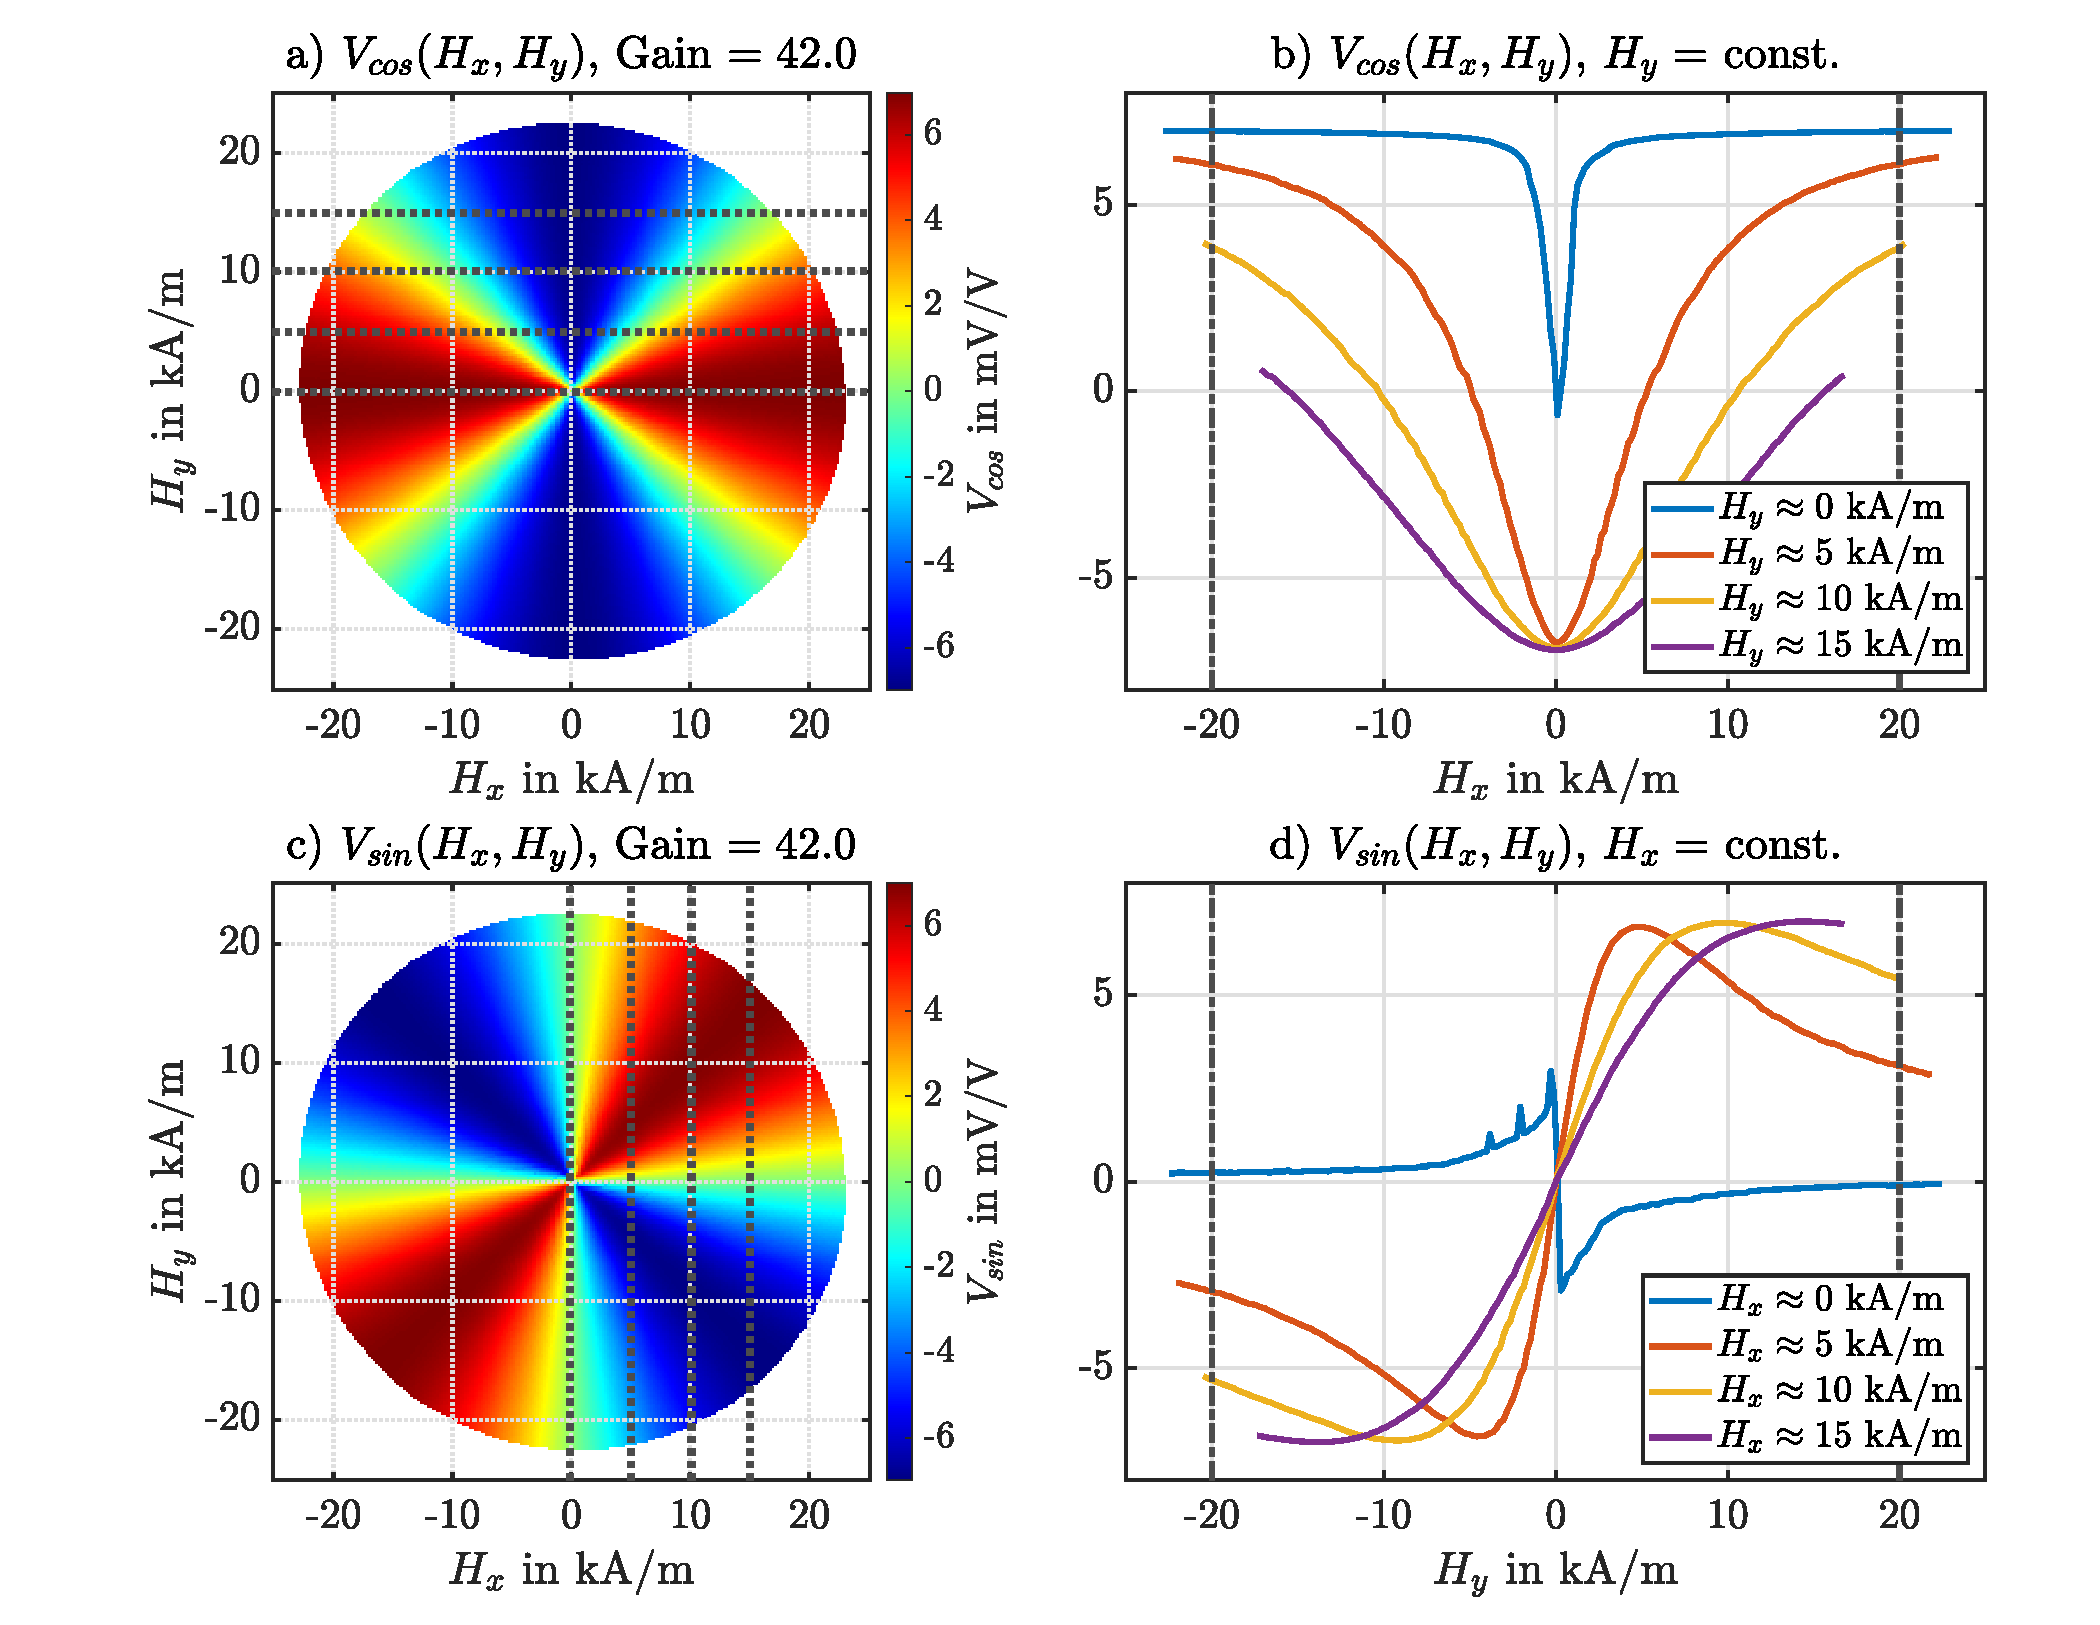
\includegraphics[width=\linewidth]{appendix/images/4-KMZ60/KMZ60_Kennfeld_Steigend}
	\caption[NXP KMZ60 Kennfeldquerschnitte]{NXP KMZ60 Kennfeldquerschnitte. Für die Kennfelder gewonnen aus 
		steigender Amplitudenmodulation a) und c). Es sind Querschnitte durch die jeweiligen Kennfelder in b) und d) 
		abgebildet. Für $V_{cos}$ a), b) verschiedene konstante $H_y$ und $V_{sin}$ c), d) entsprechend verschiedene 
		konstante $H_x$ Querschnitte. Grafik nachempfunden aus \cite{Schuethe2019}.}
	\label{fig:kmz60kennfeldsteigend}
\end{figure}




\begin{figure}[tbph]
	\centering
	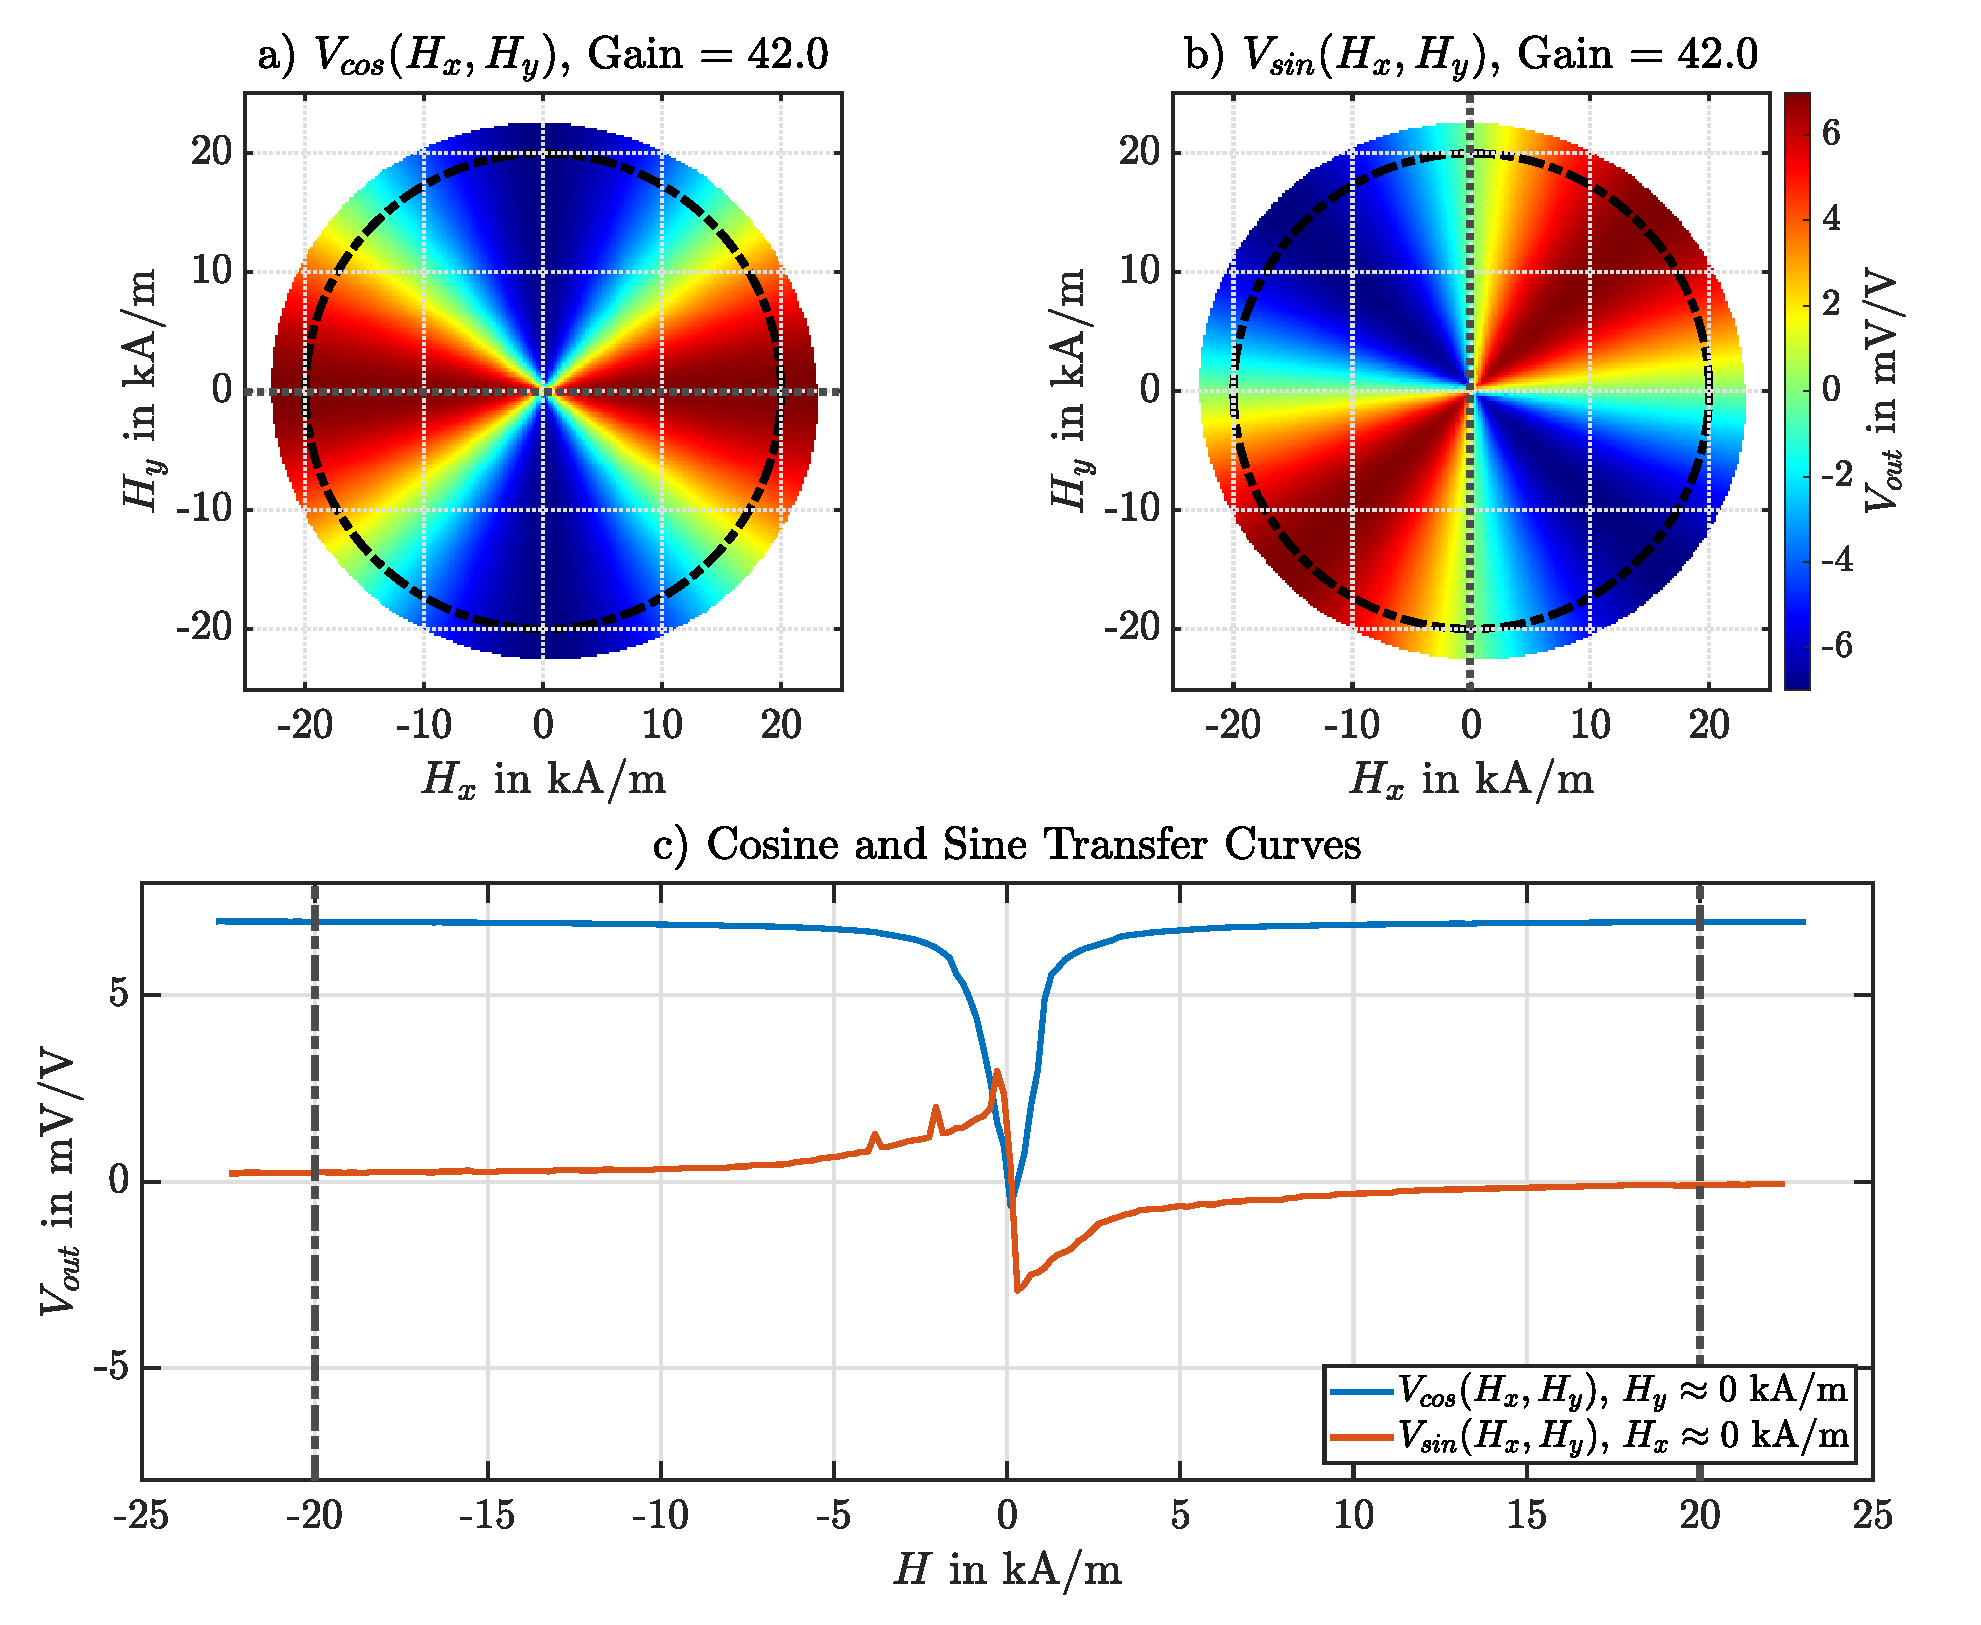
\includegraphics[width=\linewidth]{appendix/images/4-KMZ60/KMZ60_Uebertragungskennlinien}
	\caption[NXP KMZ60 Übertragungskennlinie]{NXP KMZ60 Übertragungskennlinie. Es sind wieder die Kennfelder aus 
		der steigenden Amplitudenmodulation in a) und b). In c) sind die Übertragungskennlinien für den Sensor gezeigt 
		mit Kennzeichnung für den Betrieb in Sättigung bei $\SI{20}{\kilo\ampere\per\metre}$. Ebenfalls zu sehen in a) 
		und b) durch die sich ergebene Kreisbahn mit einem Radius des aufgelegten Intervalls aus c). Grafik 
		nachempfunden aus \cite{Schuethe2019}.}
	\label{fig:kmz60uebertragungskennlinien}
\end{figure}
